\documentclass[10pt,letterpaper]{article}
% The usepackage tell LaTeX which packages are needed. As you get better you can add more
% packages for extra functionality
% Percent signs are comments, they will not be read by the renderer.
\usepackage{fullpage}
\usepackage[top=2cm, bottom=2.5cm, left=2.5cm, right=2.5cm]{geometry}
\usepackage{amsmath,amsthm,amsfonts,amssymb,amscd}
\usepackage{lastpage}
\usepackage{enumerate}
\usepackage{fancyhdr}
\usepackage{mathrsfs}
\usepackage{xcolor}
\usepackage{graphicx}
\usepackage{hyperref}
\usepackage[shortlabels]{enumitem}
\usepackage{listings} %for listings of the source code

% Some definitions for using the listing package.
% When we reference 'codegreen', it will be the RGB color defined below.
\definecolor{codegreen}{rgb}{0,0.6,0}
\definecolor{codegray}{rgb}{0.5,0.5,0.5}
\definecolor{codepurple}{rgb}{0.58,0,0.82}
\definecolor{backcolour}{rgb}{0.95,0.95,0.92}
\DeclareUnicodeCharacter{2212}{-}

% Also for the listings, this will make the code listing look like default MATLAB
\lstdefinestyle{mystyle}{
	backgroundcolor=\color{backcolour},   
	commentstyle=\color{codegreen},
	keywordstyle=\color{magenta},
	numberstyle=\tiny\color{codegray},
	stringstyle=\color{codepurple},
	basicstyle=\footnotesize,
	breakatwhitespace=false,         
	breaklines=true,                 
	captionpos=b,                    
	keepspaces=true,                 
	numbers=left,                    
	numbersep=5pt,                  
	showspaces=false,                
	showstringspaces=false,
	showtabs=false,                  
	tabsize=2
}
\lstset{style=mystyle}

\hypersetup{%
  colorlinks=true,
  linkcolor=blue,
  linkbordercolor={0 0 1}
}
 
\setlength{\parindent}{0.0in}
\setlength{\parskip}{0.05in}

\newcommand\course{COMP 521 }
\newcommand\hwnumber{2}             
\newcommand\MyName{Zack Humphries}  

\pagestyle{fancyplain}
\headheight 15pt
\lhead{\MyName}
%\lhead{\NetIDa\\\NetIDb}                 % <-- Comment this line out for problem sets (make sure you are person #1)
\chead{\textbf{\Large Homework \hwnumber}}
\rhead{\course\\ \today}
\lfoot{}
\cfoot{}
\rfoot{\small\thepage}
\headsep 1.5em

\begin{document}

%%%%%%%%%%%%%%%%%%%%%%%%%%%%%%%%%%%%%%%%%%%%%%%%%%%%%%%%%%%%%%%%%%%

\section*{Problem 1} % Note the asteric so you do not get an additional number

Calculate the centered finite difference approximation of $f''(x)$ for the following functions on the interval $x \in [-1,1]$. Show the numerical and the analytical results in the same plot using a grid size h = 0.02. Show the log-log plots of the errors versus grid sizes. Use at least 4 grid sizes for the error plot

%%%%%%%%%%%%%%%%%%%%%%%%%%%%%%%%%%%%%%%%%%%%%%%%%%%%%%%%%%%%%%%%%%%

As requested, the initial values are h = 0.02, an interval of $[-1,1]$ with interval gaps of h. Finally grid\_size = 4

\lstset{title={Initialization}}
\begin{lstlisting}[language = Matlab]
h = 0.02;                       % sets h
number_of_grids = 4;            % grid sizes for error plot
x_interval = -1+h : h : 1-h;    % sets interval [-1 to 1] for xi with h gap
\end{lstlisting}

\begin{enumerate}[a)]
  \item 
  $f(x) = e^x \sin(\frac{\pi x}{2})$


    Described in the function, problem\_1\_f(x):
    
    \lstset{title={problem\_1\_f(x)}}
      \begin{lstlisting}[language = Matlab]
function result = problem_1_f(x)
    result = exp(x)*sin((pi*x)/2);  % Returns f(x) for Problem A
end \end{lstlisting}
    
    The actual second derivative of $f(x)$ is\ldots

    \makebox[\textwidth]{$f''(x) = \frac{-1}{4} e^x [(\pi ^2-4) \sin(\frac{\pi x}{2})-4 \pi \cos(\frac{\pi x}{2})]$}

    Described in the function, problem\_1\_f\_double\_prime(x):
    \lstset{title={problem\_1\_f\_double\_prime(x)}}
     \begin{lstlisting}[language = Matlab]
function result = problem_1_f_double_prime(x)
    result = -(1/4) * exp(x)*(((pi^2)-4)*sin(pi*x/2)-4*pi*cos(pi*x/2)); % Returns actual f"(x) for Problem A
end \end{lstlisting}


    However using the 2nd derivative centered difference approximation:
    
    \makebox[\textwidth]{$f''(x_{i}) \approx  u''_i = \frac{u_{i+1}-2u_{i}+u_{i-1}}{h^2}$}
    
    We can also approximate the second derivative. The 2nd derivative centered difference approximation is described in the function, f\_double\_prime(ui\_plus,ui,ui\_minus,h):

    \lstset{title={f\_double\_prime(ui\_plus,ui,ui\_minus,h)}}
     \begin{lstlisting}[language = Matlab]
function result = f_double_prime(ui_plus,ui,ui_minus,h)
    result = (ui_plus - (2*ui) + ui_minus)/(h^2);   % centered finite difference approximation of f"(x)
end\end{lstlisting}


    In order to get all of the estimated and actual $f''(x_{i})$ values, we call the problem\_1(x\_interval,h) function.
    The problem\_1(x\_interval,h) function takes the inputs, x\_interval and h, which were initialized beforehand. The function returns\ldots 
    \begin{enumerate}
      \item estimate\_interval: an array of estimated $f''(x)$ values (based off of the 2nd derivative centered difference approximation)
      \item actual\_interval: an array of actual $f''(x)$ values
      \item estimate\_middle: the value of the element in the center/middle of estimate\_interval (to be used later for log-log plots)
      \item actual\_middle: the value of the element in the center/middle of actual\_interval (to be used later for log-log plots)
    \end{enumerate}
    \lstset{title={calling problem\_1(x\_interval,h)}}
     \begin{lstlisting}[language = Matlab]
[estimate_interval, actual_interval,estimate_middle,actual_middle] = ...
problem_1(x_interval,h);    % returns estimate vs actual and middle estimate vs actual for reference
\end{lstlisting}
    \lstset{title={problem\_1(x\_interval,h)}}
     \begin{lstlisting}[language = Matlab]
function [estimate_interval, actual_interval,estimate_middle,actual_middle] = ...
      problem_1(interval,h)                       % Problem A
  interval_length = length(interval);             % saves number of xi's in x_interval
  estimate_interval = zeros(1,length(interval));  % makes empty array for estimate f"(x)
  actual_interval = zeros(1,length(interval));    % makes empty array for actual f"(x)
  for n=1:interval_length
      xi = interval(n);                           % goes through each xi
      ui = problem_1_f(xi);                       % returns f(xi) for f"(xi) estimation
      ui_plus = problem_1_f(xi + h);              % returns f(xi+h) for f"(xi) estimation
      ui_minus = problem_1_f(xi - h);             % returns f(xi+h) for f"(xi) estimation
      estimate_interval(n) = f_double_prime(ui_plus,ui,ui_minus,h);   % estimate f"(xi)
      actual_interval(n) = problem_1_f_double_prime(xi);              % actual f"(xi)
  end
  estimate_middle = estimate_interval((interval_length+1)/2);         % since x_interval will always have an odd number of values,
  actual_middle = actual_interval((interval_length+1)/2);             % (interval_length+1)/2 will always return middle estimate/actual
end
\end{lstlisting}

    Plotting the estimate and actual intervals against x\_interval, we get\ldots
    \begin{figure}[h!]
      \centering
      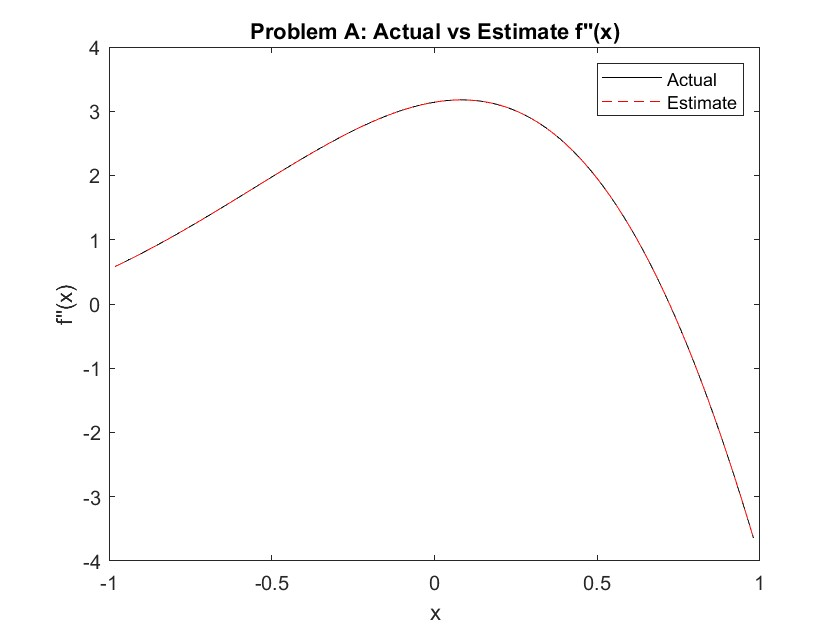
\includegraphics[width=0.75\linewidth]{problem_a_estimate_vs_actual.jpg}
      \caption{Problem A\: Actual vs Estimate $f''(x)$}\label{fig:problem_a_estimate_vs_actual}
    \end{figure}

    \lstset{title={Plotting Problem A}}
     \begin{lstlisting}[language = Matlab]
% Plotting Problem A: Actual vs Estimate f''(x)
plot(x_interval, actual_interval, 'k-')
hold on;
plot(x_interval, estimate_interval, 'r--')
legend("Actual", "Estimate")
xlabel("x")
ylabel("f``(x)")
title("Problem A: Actual vs Estimate f``(x)")
hold off
\end{lstlisting}
    
    In order to display the log-log plot, we call the grid\_reduction(h, number\_of\_grids, problem\_number), which takes in h, the number of grids, and the problem number (1 for A and 2 for B). It returns\ldots 
    \begin{enumerate}
      \item h\_interval: an array of all h intervals (ex. [$h, \frac{h}{2}, \frac{h}{4}, \frac{h}{8},\ldots$])
      \item error\_list: the error approximation for each $\frac{h}{2^n}$. 
    \end{enumerate}

    \lstset{title={calling grid\_reduction(h, number\_of\_grids, problem\_number)}}
     \begin{lstlisting}[language = Matlab]
problem_number = 1; % 1 for Problem A
[h_interval, error_list] = grid_reduction(h,number_of_grids, problem_number);
    \end{lstlisting}
    \lstset{title={grid\_reduction(h, number\_of\_grids, problem\_number)}}
     \begin{lstlisting}[language = Matlab]
function [h_interval, error_list] = grid_reduction(h,number_of_grids, problem_number)
  h_interval = zeros(1,number_of_grids);      % sets empty array for future h/# values
  error_list = zeros(1,number_of_grids);      % sets empty array for error approximations
  h_div = h;                                  % initializes first h = h
  for n=1:number_of_grids
      h_interval(n) = h_div;                  % replaces 0 in empty array with actual h/# value
      interval = -1+h_div : h_div : 1-h_div;  % makes fresh xi interval with h/# as gap
      if problem_number == 1      % If problem A, returns estimate vs actual for each xi based on h/# gap AND estimate and actual middle value for loglog graph
          [estimate_interval, actual_interval,estimate_middle,actual_middle] = ...
              problem_1(interval,h_div);
      elseif problem_number == 2  % If problem B...
          [estimate_interval, actual_interval,estimate_middle,actual_middle] = ...
              problem_2(interval,h_div);
      end
      error = (abs(estimate_middle-actual_middle))^(1.0/number_of_grids); % error approximation
      error_list(n) = error;                  % replaces 0 in empty error_list array with error approximation
      h_div = h/(2^n);                        % sets new h value (h/(2^grid_size))
  end
end
\end{lstlisting}
    
\pagebreak
    We can then create the log-log plot with respect to h\_interval and error\_list\ldots
    \begin{figure}[h!]
      \centering
      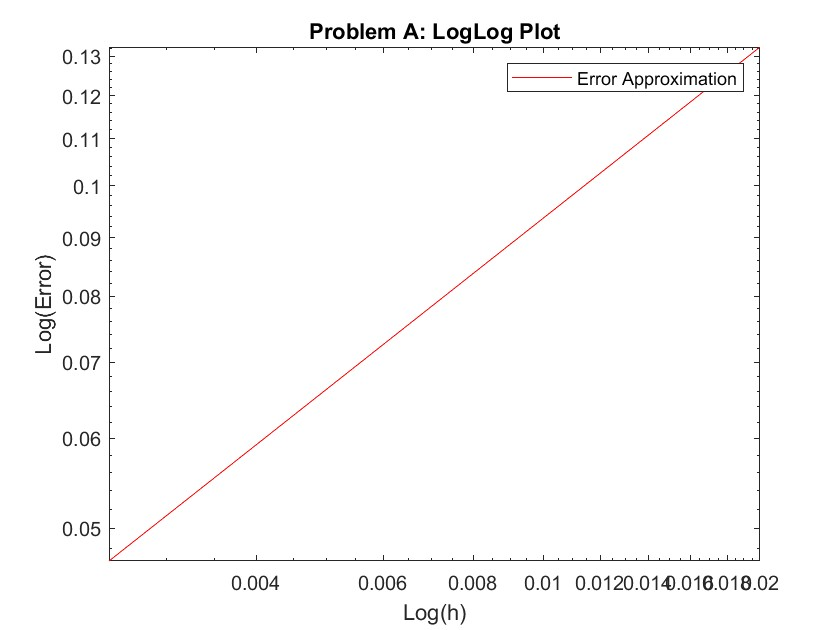
\includegraphics[width=1\linewidth]{problem_a_loglog_plot.jpg}
      \caption{Problem A\: LogLog Plot}\label{fig:problem_a_loglog_plot}
    \end{figure}

    \lstset{title={Plotting Problem A\: LogLog Plot}}
     \begin{lstlisting}[language = Matlab]
% Plotting Problem A: LogLog Plot
figure(2)
loglog(h_interval, error_list, 'r-')
legend("Error Approximation")
xlabel("Log(h)")
ylabel("Log(Error)")
title("Problem A: LogLog Plot")
hold off
    \end{lstlisting}
    
\pagebreak
  \item
    $f(x) = 2 \cos^2(\pi x) -1$

    Described in the function, problem\_2\_f(x):
    
    \lstset{title={problem\_2\_f(x)}}
      \begin{lstlisting}[language = Matlab]
function result = problem_2_f(x)
    result = 2*(cos(pi*x)^2)-1;  % Returns f(x) for Problem B
end \end{lstlisting}

    The actual second derivative of f(x) is\ldots

    \makebox[\textwidth]{$f''(x) = 4\pi^2 [(\sin^2(\pi x))-(\cos^2(\pi x))] $}
    Described in the function, problem\_2\_f\_double\_prime(x):
    \lstset{title={problem\_2\_f\_double\_prime(x)}}
     \begin{lstlisting}[language = Matlab]
function result = problem_2_f_double_prime(x)
    result = 4*(pi^2)*((sin(pi*x)^2)-(cos(pi*x)^2)); % Returns actual f"(x) for Problem B
end \end{lstlisting}
    
    However using the 2nd derivative centered difference approximation:
    
    \makebox[\textwidth]{$f''(x_{i}) \approx  u''_i = \frac{u_{i+1}-2u_{i}+u_{i-1}}{h^2}$}
    
    We can again approximate the second derivative.

    Problem B works exactly like Problem A at this point, except using a different function, problem\_1(x\_interval,h) to solve for $f''(x_i)$. Only thing different is that it calls problem\_2\_f(xi) and problem\_2\_f\_double\_prime(xi).
    \lstset{title={problem\_2\_f\_double\_prime(x)}}
     \begin{lstlisting}[language = Matlab]
function [estimate_interval, actual_interval,estimate_middle,actual_middle] = ...
        problem_2(interval,h)                       % Problem B
    interval_length = length(interval);             % ...
    estimate_interval = zeros(1,length(interval));
    actual_interval = zeros(1,length(interval));
    for n=1:interval_length
        xi = interval(n);
        ui = problem_2_f(xi);
        ui_plus = problem_2_f(xi + h);
        ui_minus = problem_2_f(xi - h);
        estimate_interval(n) = f_double_prime(ui_plus,ui,ui_minus,h);
        actual_interval(n) = problem_2_f_double_prime(xi);
    end
    estimate_middle = estimate_interval((interval_length+1)/2);
    actual_middle = actual_interval((interval_length+1)/2);
end\end{lstlisting}

\pagebreak
    The actual vs estimate plot for Problem B looks like \ldots
    \begin{figure}[h!]
      \centering
      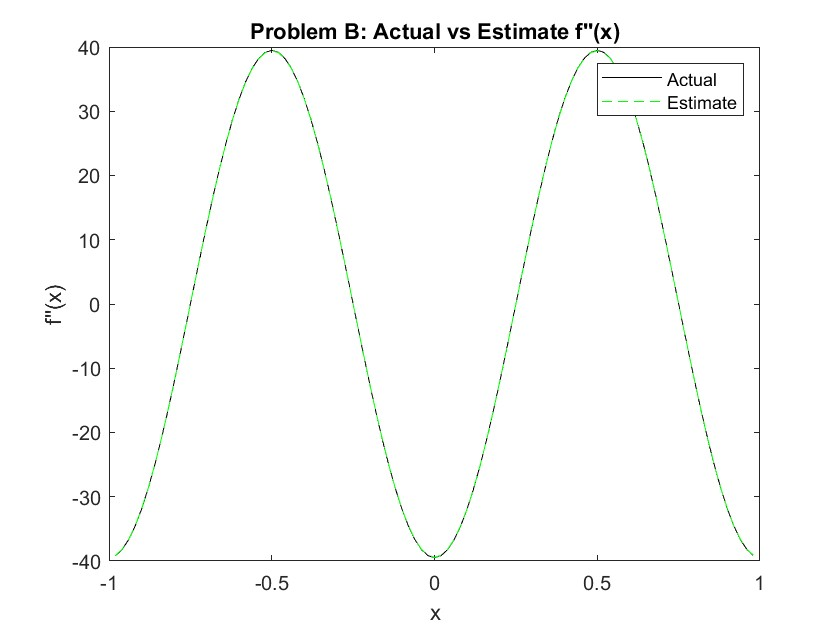
\includegraphics[width=0.75\linewidth]{problem_b_estimate_vs_actual.jpg}
      \caption{Problem B\: Actual vs Estimate $f''(x)$}\label{fig:problem_b_estimate_vs_actual}
    \end{figure}
    \lstset{title={Plotting Problem A}}
     \begin{lstlisting}[language = Matlab]

% Plotting Problem B: Actual vs Estimate f''(x)
figure(3)
plot(x_interval, actual_interval, 'k-')
hold on;
plot(x_interval, estimate_interval, 'g--')
legend("Actual", "Estimate")
xlabel("x")
ylabel("f``(x)")
title("Problem B: Actual vs Estimate f``(x)")
hold off
\end{lstlisting}

\pagebreak
The LogLog plot for Problem B looks like \ldots

\begin{figure}[h!]
  \centering
  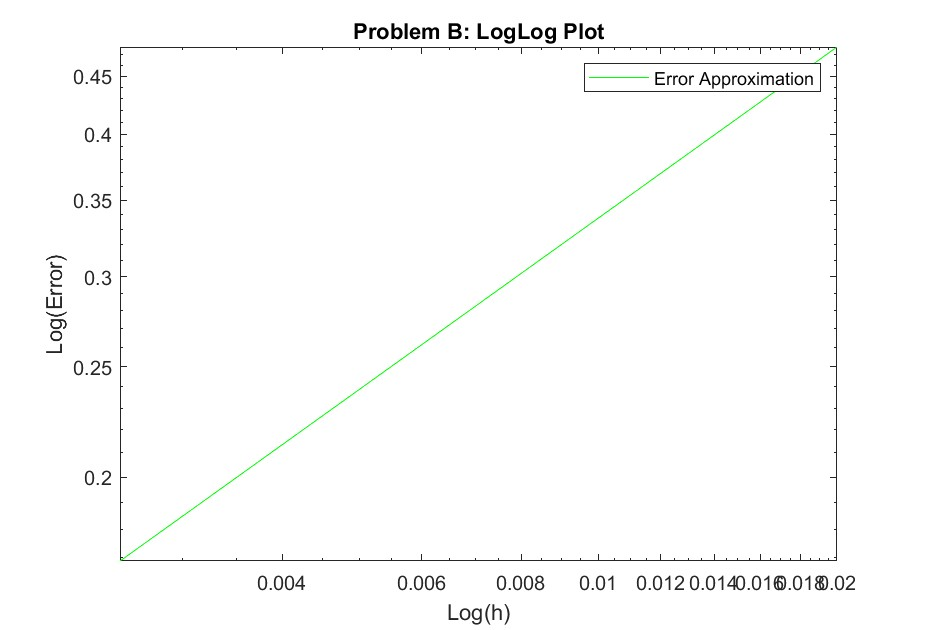
\includegraphics[width=0.75\linewidth]{problem_b_loglog_plot.jpg}
  \caption{Problem B\: LogLog Plot}\label{fig:problem_b_loglog_plot}
\end{figure}


\lstset{title={Plotting Problem B\: LogLog Plot}}
 \begin{lstlisting}[language = Matlab]
problem_number = 2; % 2 for Problem B
[h_interval, error_list] = grid_reduction(h,number_of_grids, problem_number);

% Plotting Problem B: LogLog Plot
figure(4)
loglog(h_interval, error_list, 'g-')
legend("Error Approximation")
xlabel("Log(h)")
ylabel("Log(Error)")
title("Problem B: LogLog Plot")
hold off
\end{lstlisting}

\end{enumerate}

\pagebreak

\lstset{title={Homework 2}}
 \begin{lstlisting}[language = Matlab]
%% Zack Humphries
% COMP 521
% HW2

clc;       % clear command window
clear;     % removes all saved variables
close all; % close any open windows

%%
h = 0.02;               % sets h
number_of_grids = 4;    % grid sizes for error plot
x_interval = -1+h : h : 1-h;    % sets interval [-1 to 1] for xi with h gap

%% Problem A
[estimate_interval, actual_interval,estimate_middle,actual_middle] = ...
    problem_1(x_interval,h);    % returns estimate vs actual and middle estimate vs actual for reference

% Plotting Problem A: Actual vs Estimate f''(x)
plot(x_interval, actual_interval, 'k-')
hold on;
plot(x_interval, estimate_interval, 'r--')
legend("Actual", "Estimate")
xlabel("x")
ylabel("f``(x)")
title("Problem A: Actual vs Estimate f``(x)")
hold off


% Returns all h intervals (ex. [h, h/2, h/4, h/8,...]) and the error
% approximation for each h/(2^n). Takes in problem_number (1 for A and 2
% for B)
problem_number = 1; % 1 for Problem A
[h_interval, error_list] = grid_reduction(h,number_of_grids, problem_number);

% Plotting Problem A: LogLog Plot
figure(2)
loglog(h_interval, error_list, 'r-')
legend("Error Approximation")
xlabel("Log(h)")
ylabel("Log(Error)")
title("Problem A: LogLog Plot")
hold off

%% Problem B
[estimate_interval, actual_interval,estimate_middle,actual_middle] = ...
    problem_2(x_interval,h);

% Plotting Problem B: Actual vs Estimate f''(x)
figure(3)
plot(x_interval, actual_interval, 'k-')
hold on;
plot(x_interval, estimate_interval, 'g--')
legend("Actual", "Estimate")
xlabel("x")
ylabel("f``(x)")
title("Problem B: Actual vs Estimate f``(x)")
hold off

problem_number = 2; % 2 for Problem B
[h_interval, error_list] = grid_reduction(h,number_of_grids, problem_number);

% Plotting Problem B: LogLog Plot
figure(4)
loglog(h_interval, error_list, 'g-')
legend("Error Approximation")
xlabel("Log(h)")
ylabel("Log(Error)")
title("Problem B: LogLog Plot")
hold off

%% Functions used for calculations
function [h_interval, error_list] = grid_reduction(h,number_of_grids, problem_number)
    h_interval = zeros(1,number_of_grids);      % sets empty array for future h/# values
    error_list = zeros(1,number_of_grids);      % sets empty array for error approximations
    h_div = h;                                  % initializes first h = h
    for n=1:number_of_grids
        h_interval(n) = h_div;                  % replaces 0 in empty array with actual h/# value
        interval = -1+h_div : h_div : 1-h_div;  % makes fresh xi interval with h/# as gap
        if problem_number == 1      % If problem A, returns estimate vs actual for each xi based on h/# gap AND estimate and actual middle value for loglog graph
            [estimate_interval, actual_interval,estimate_middle,actual_middle] = ...
                problem_1(interval,h_div);
        elseif problem_number == 2  % If problem B...
            [estimate_interval, actual_interval,estimate_middle,actual_middle] = ...
                problem_2(interval,h_div);
        end
        error = (abs(estimate_middle-actual_middle))^(1.0/number_of_grids); % error approximation
        error_list(n) = error;                  % replaces 0 in empty error_list array with error approximation
        h_div = h/(2^n);                        % sets new h value (h/(2^grid_size))
    end
end

function [estimate_interval, actual_interval,estimate_middle,actual_middle] = ...
        problem_1(interval,h)                       % Problem A
    interval_length = length(interval);             % saves number of xi's in x_interval
    estimate_interval = zeros(1,length(interval));  % makes empty array for estimate f"(x)
    actual_interval = zeros(1,length(interval));    % makes empty array for actual f"(x)
    for n=1:interval_length
        xi = interval(n);                           % goes through each xi
        ui = problem_1_f(xi);                       % returns f(xi) for f"(xi) estimation
        ui_plus = problem_1_f(xi + h);              % returns f(xi+h) for f"(xi) estimation
        ui_minus = problem_1_f(xi - h);             % returns f(xi+h) for f"(xi) estimation
        estimate_interval(n) = f_double_prime(ui_plus,ui,ui_minus,h);   % estimate f"(xi)
        actual_interval(n) = problem_1_f_double_prime(xi);              % actual f"(xi)
    end
    estimate_middle = estimate_interval((interval_length+1)/2);         % since x_interval will always have an odd number of values,
    actual_middle = actual_interval((interval_length+1)/2);             % (interval_length+1)/2 will always return middle estimate/actual
end

function [estimate_interval, actual_interval,estimate_middle,actual_middle] = ...
        problem_2(interval,h)                       % Problem B
    interval_length = length(interval);             % ...
    estimate_interval = zeros(1,length(interval));
    actual_interval = zeros(1,length(interval));
    for n=1:interval_length
        xi = interval(n);
        ui = problem_2_f(xi);
        ui_plus = problem_2_f(xi + h);
        ui_minus = problem_2_f(xi - h);
        estimate_interval(n) = f_double_prime(ui_plus,ui,ui_minus,h);
        actual_interval(n) = problem_2_f_double_prime(xi);
    end
    estimate_middle = estimate_interval((interval_length+1)/2);
    actual_middle = actual_interval((interval_length+1)/2);
end

function result = f_double_prime(ui_plus,ui,ui_minus,h)
    result = (ui_plus - (2*ui) + ui_minus)/(h^2);   % centered finite difference approximation of f"(x)
end

function result = problem_1_f(x)
    result = exp(x)*sin((pi*x)/2);  % Returns f(x) for Problem A
end

function result = problem_1_f_double_prime(x)
    result = -(1/4) * exp(x)*(((pi^2)-4)*sin(pi*x/2)-4*pi*cos(pi*x/2)); % Returns actual f"(x) for Problem A
end

function result = problem_2_f(x)
    result = 2*(cos(pi*x)^2)-1;  % Returns f(x) for Problem B
end

function result = problem_2_f_double_prime(x)
    result = 4*(pi^2)*((sin(pi*x)^2)-(cos(pi*x)^2)); % Returns actual f"(x) for Problem B
end
\end{lstlisting}

\end{document}
